\usetikzlibrary{calc}
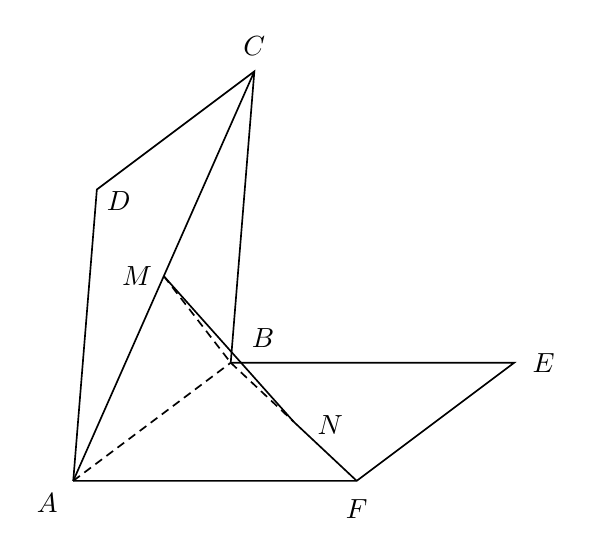
\begin{tikzpicture}[x=1cm,y=1cm,line width=.6pt,font=\normalsize]
\coordinate (A) at (0,0);
\coordinate (B) at (2.0,1.5);
\coordinate (C) at (2.3,5.2);
\coordinate (D) at (0.3000000000,3.7000000000);
\coordinate (E) at (5.6000000000,1.5000000000);
\coordinate (F) at (3.6,0);
\coordinate (M) at (1.1500000000,2.6000000000);
\coordinate (N) at (2.8000000000,0.7500000000);
% square ABCD (left/up): A-D-D-C-C-B solid, A-B dashed hinge
\draw (A) -- (D) -- (C) -- (B);
\draw[densely dashed] (A) -- (B);
% diagonal AC solid through M
\draw (A) -- (C);
% square ABEF (right): A-F, F-E, E-B solid, A-B dashed
\draw (A) -- (F) -- (E) -- (B);
% diagonal BF with N: B-N dashed, N-F solid
\draw[densely dashed] (B) -- (N);
\draw (N) -- (F);
% segments MA/MB/MN for dihedral illustration
\draw[densely dashed] (M)--(B);
\draw (M) -- (N);
% C-B vertical solid already drawn; C-M part of AC
% labels
\node[anchor=north east,xshift=-2pt,yshift=-1pt] at (A) {$A$};
\node[anchor=west,xshift=4pt,yshift=9pt] at (B) {$B$};
\node[anchor=south,yshift=2pt] at (C) {$C$};
\node[anchor=west,xshift=0pt,yshift=-4pt] at (D) {$D$};
\node[anchor=west,xshift=3pt] at (E) {$E$};
\node[anchor=north,yshift=-3pt] at (F) {$F$};
\node[left=3pt,inner sep=1pt] at (M) {$M$};
\node[anchor=west,xshift=5pt,yshift=-1pt] at (N) {$N$};
\end{tikzpicture}
